
\definecolor{c746c66}{RGB}{116,108,102}


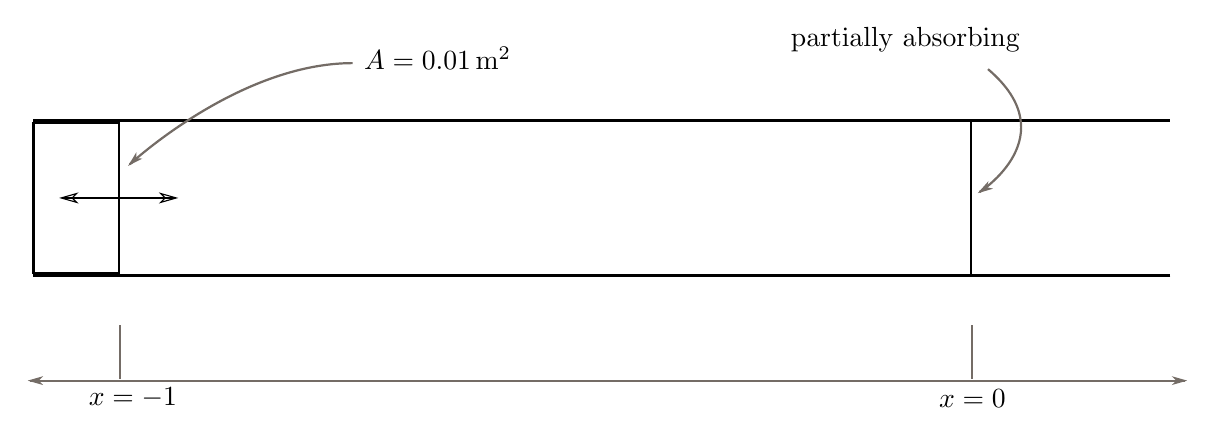
\begin{tikzpicture}[y=0.80pt, x=0.8pt,yscale=-1, inner sep=0pt, outer sep=0pt]
\begin{scope}[shift={(0,-872.35975)}]
  \begin{scope}[fill=c746c66]
    \path[color=black,fill=c746c66,line width=0.800pt] (9.8750,1034.3598) --
      (9.8750,1035.3598) -- (531.6250,1035.3598) -- (531.6250,1034.3598) --
      (9.8750,1034.3598) -- cycle;
    \path[fill=c746c66,even odd rule,line width=0.400pt] (13.8873,1034.8668) --
      (15.8873,1032.8668) -- (8.8873,1034.8668) -- (15.8873,1036.8668) --
      (13.8873,1034.8668) -- cycle;
    \path[fill=c746c66,even odd rule,line width=0.400pt] (527.6338,1034.8668) --
      (525.6338,1036.8668) -- (532.6338,1034.8668) -- (525.6338,1032.8668) --
      (527.6338,1034.8668) -- cycle;
  \end{scope}
  \path[color=black,fill=c746c66,line width=0.800pt] (435.0000,1009.7812) --
    (435.0000,1034.0938) -- (436.0000,1034.0938) -- (436.0000,1009.7812) --
    (435.0000,1009.7812) -- cycle;
  \path[shift={(0,872.35975)},fill=black] (416.02817,176.95775) node[above right]
    (text2989) {};
  \path[fill=c746c66] (420.59155,1047.0358) node[above right] (text2993) {$x=0$};
  \path[shift={(0,872.35975)},draw=black,line join=miter,line cap=butt,line
    width=0.800pt] (11.5000,115.0000) -- (435.0000,115.0000) -- (435.0000,45.0000)
    -- (11.5000,45.0000);
  \path[shift={(0,872.35975)},draw=black,line join=miter,line cap=butt,line
    width=0.800pt] (525.0000,115.0000) -- (435.0000,115.0000) --
    (435.0000,45.0000) -- (525.0000,45.0000);
  \path[shift={(0,872.35975)},fill=c746c66] (353.66196,14.197183) node[above
    right] (text3001) {partially absorbing};
  \begin{scope}[fill=c746c66]
    \path[color=black,fill=c746c66,line width=0.800pt] (442.9688,893.7972) --
      (442.3125,894.5472) .. controls (451.1886,902.1014) and (455.3634,909.2669) ..
      (456.6562,915.7660) .. controls (457.9491,922.2651) and (456.3887,928.1446) ..
      (453.7188,933.1097) .. controls (448.3789,943.0400) and (438.5625,949.2660) ..
      (438.5625,949.2660) -- (439.1250,950.1097) .. controls (439.1250,950.1097) and
      (449.0956,943.8031) .. (454.5938,933.5785) .. controls (457.3428,928.4662) and
      (458.9704,922.3417) .. (457.6250,915.5785) .. controls (456.2796,908.8153) and
      (451.9659,901.4544) .. (442.9688,893.7972) -- cycle;
    \path[fill=c746c66,even odd rule,line width=0.400pt] (442.2224,947.5404) --
      (442.8394,944.7801) -- (438.0007,950.2195) -- (444.9827,948.1574) --
      (442.2224,947.5404) -- cycle;
  \end{scope}
  \path[shift={(0,872.35975)},draw=black,line join=miter,line cap=butt,miter
    limit=4.00,line width=0.800pt] (11.5000,46.0000) -- (50.0000,46.0000) --
    (50.0000,114.0000) -- (11.5000,114.0000) -- cycle;
    \path[color=black,fill=black,line width=0.800pt] (50.0000,951.8597) --
      (50.0000,952.8597) -- (75.0000,952.8597) -- (75.0000,951.8597) --
      (50.0000,951.8597) -- cycle;
    \path[draw=black,even odd rule,line width=0.400pt] (71.0000,952.3597) --
      (69.0000,954.3597) -- (76.0000,952.3597) -- (69.0000,950.3597) --
      (71.0000,952.3597) -- cycle;
    \path[color=black,fill=black,line width=0.800pt] (25.0000,951.8750) --
      (25.0000,952.8750) -- (50.0000,952.8750) -- (50.0000,951.8750) --
      (25.0000,951.8750) -- cycle;
    \path[draw=black,even odd rule,line width=0.400pt] (29.0000,952.3597) --
      (31.0000,950.3597) -- (24.0000,952.3597) -- (31.0000,954.3597) --
      (29.0000,952.3597) -- cycle;
  \path[color=black,fill=c746c66,line width=0.800pt] (50.0000,1009.7812) --
    (50.0000,1034.0938) -- (51.0000,1034.0938) -- (51.0000,1009.7812) --
    (50.0000,1009.7812) -- cycle;
  \path[fill=c746c66] (36.507046,1047.0358) node[above right] (text4426) {$x=-1$};
  \begin{scope}[fill=c746c66]
    \path[color=black,fill=c746c66,line width=0.800pt] (155.6875,890.9535) ..
      controls (103.8804,890.9535) and (54.6562,936.8285) .. (54.6562,936.8285) --
      (55.3125,937.5472) .. controls (55.3125,937.5472) and (104.4721,891.9535) ..
      (155.6875,891.9535) -- (155.6875,890.9535) -- cycle;
    \path[fill=c746c66,even odd rule,line width=0.400pt] (57.9139,934.4598) --
      (58.0173,931.6332) -- (54.2514,937.8637) -- (60.7404,934.5632) --
      (57.9139,934.4598) -- cycle;
  \end{scope}
  \path[shift={(0,872.35975)},fill=c746c66] (160.90031,21.993568) node[above
    right] (text4818) {$A=0.01\,\mathrm{m^{2}}$};
\end{scope}

\end{tikzpicture}
